\section{Principled Bandit Algorithms}

% --- Optimism in the Face of Uncertainty: keep both image slides, they're conceptually clean ---
\begin{frame}{Optimism in the Face of Uncertainty}
\centering
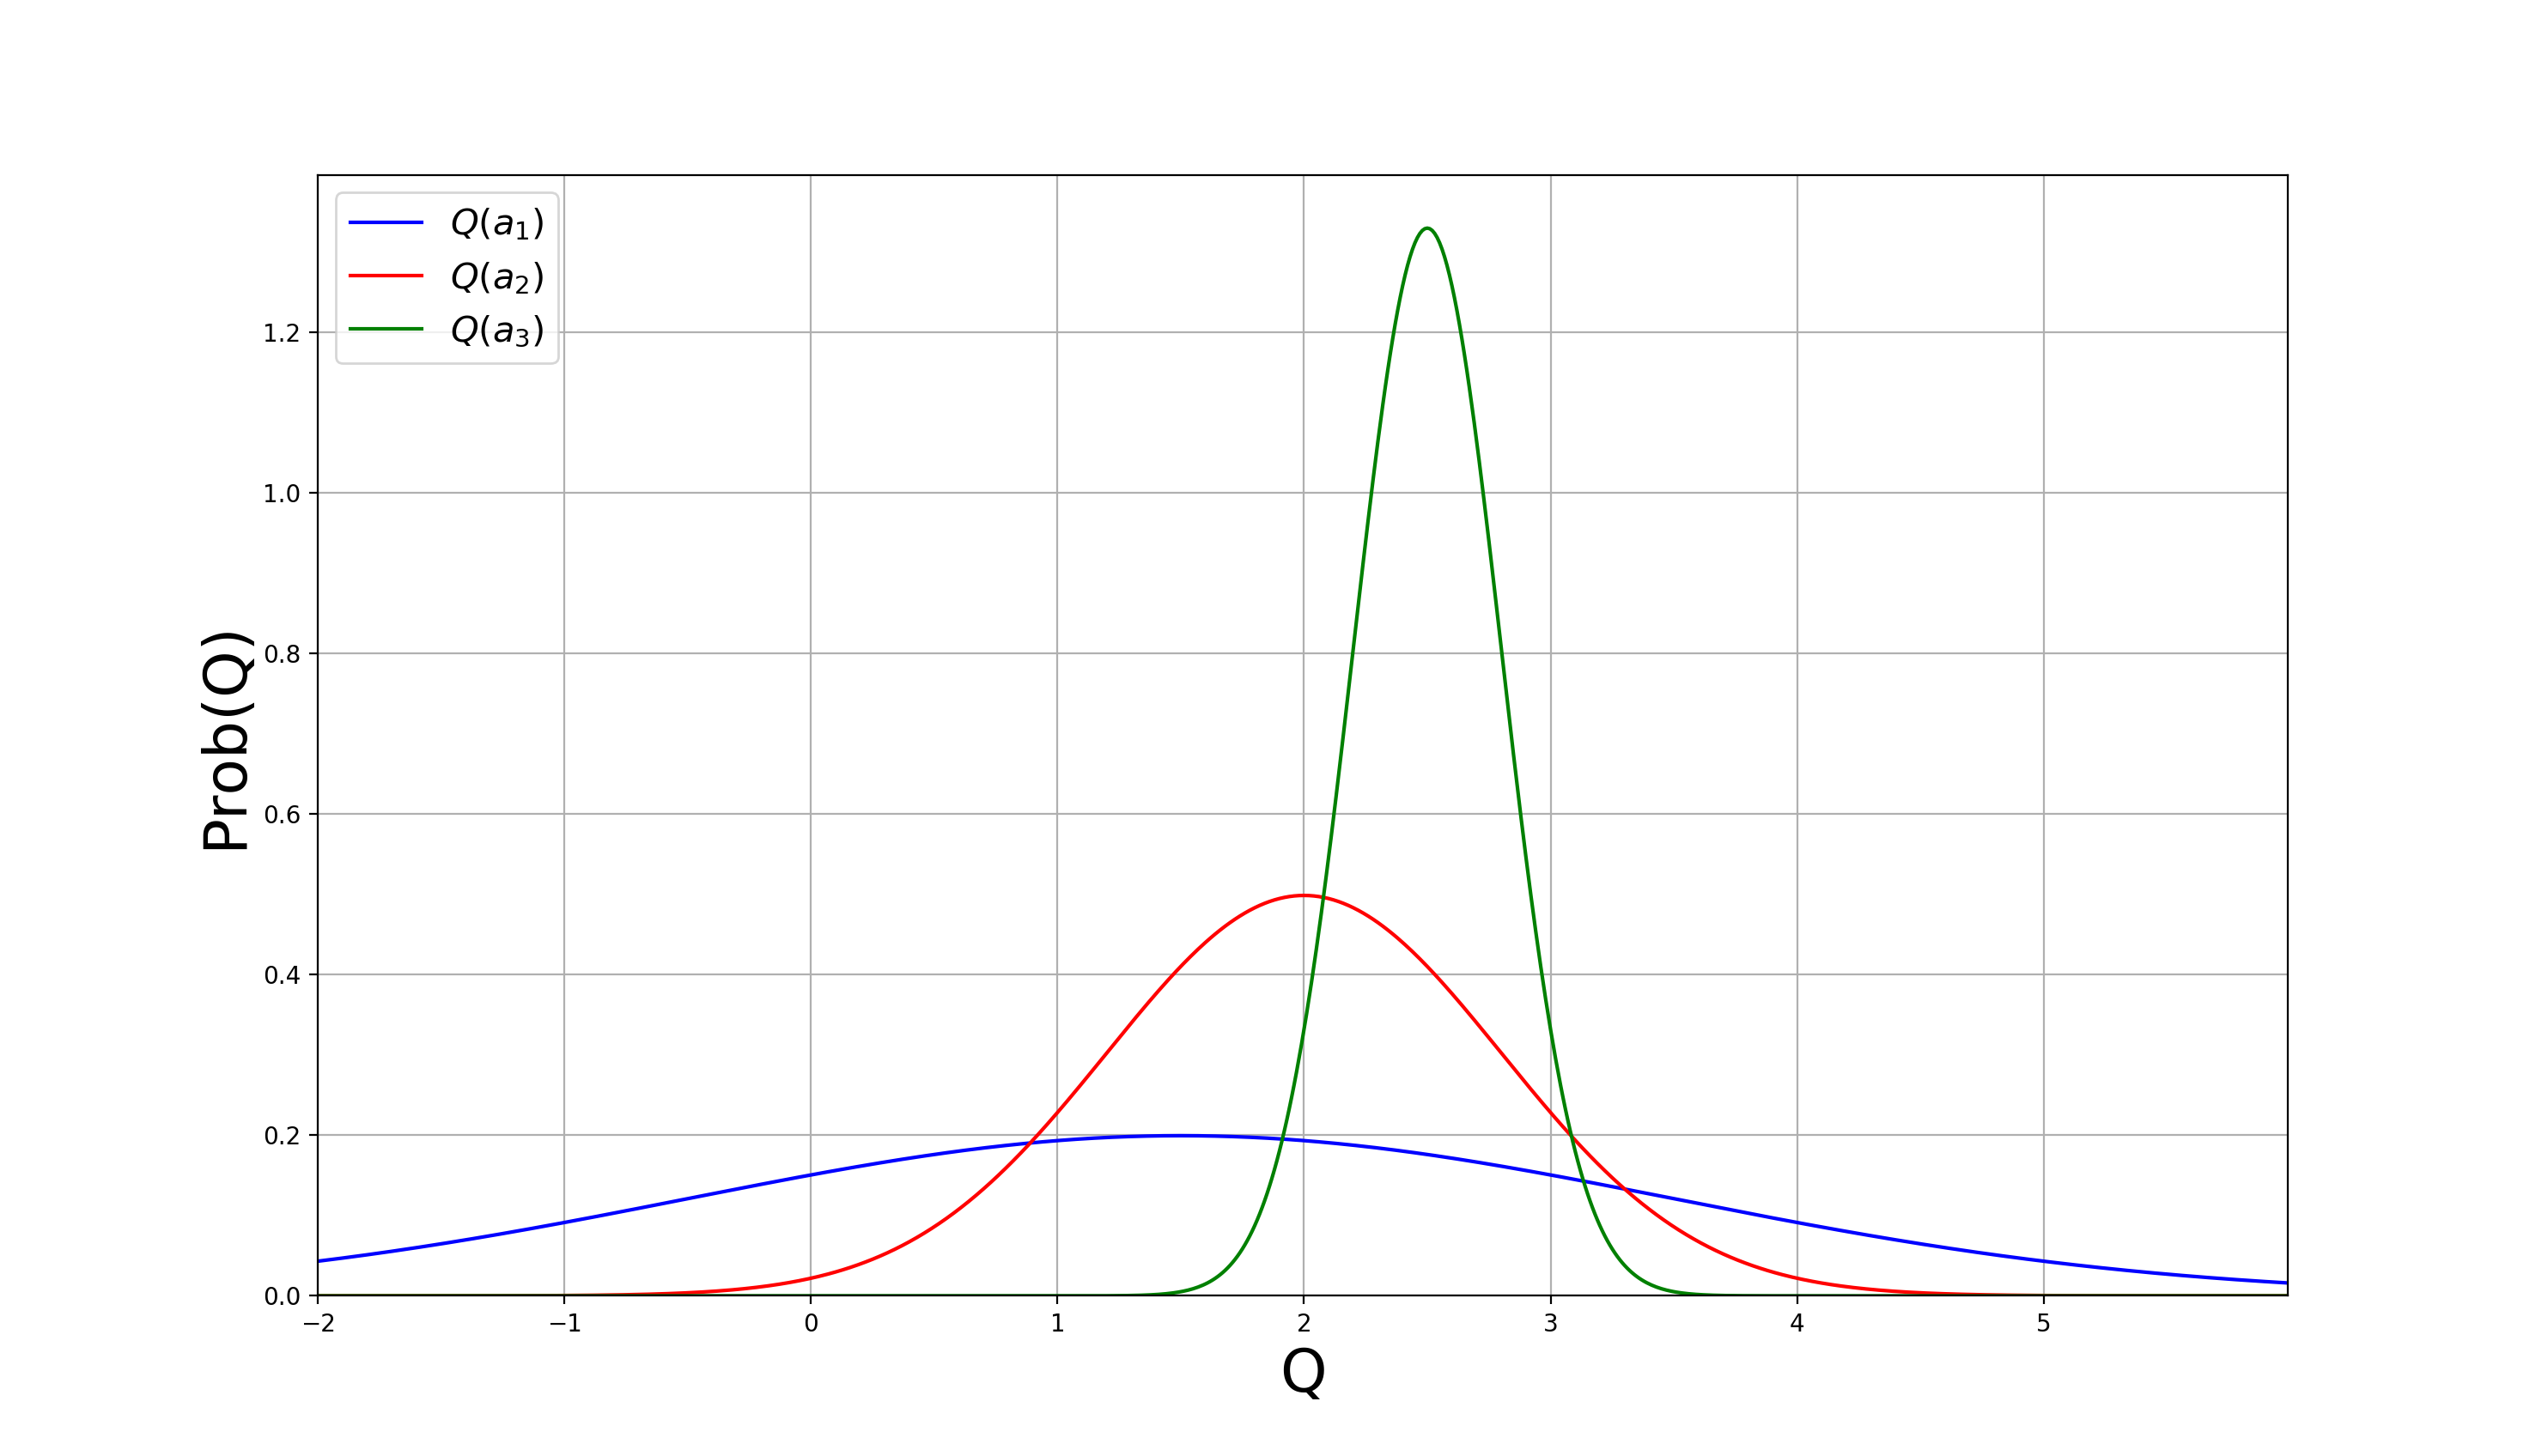
\includegraphics[width=0.62\textwidth,height=0.52\textheight,keepaspectratio]{images/bandits/figures/uncertainty-1.jpg}
\begin{itemize}
    \item Which action should we pick?
    \item \textcolor{red}{The more uncertain we are about an action-value, the more important it is to explore that action} --- it could turn out to be the best.
\end{itemize}
\end{frame}

\begin{frame}{Optimism: After One Pull}
\centering
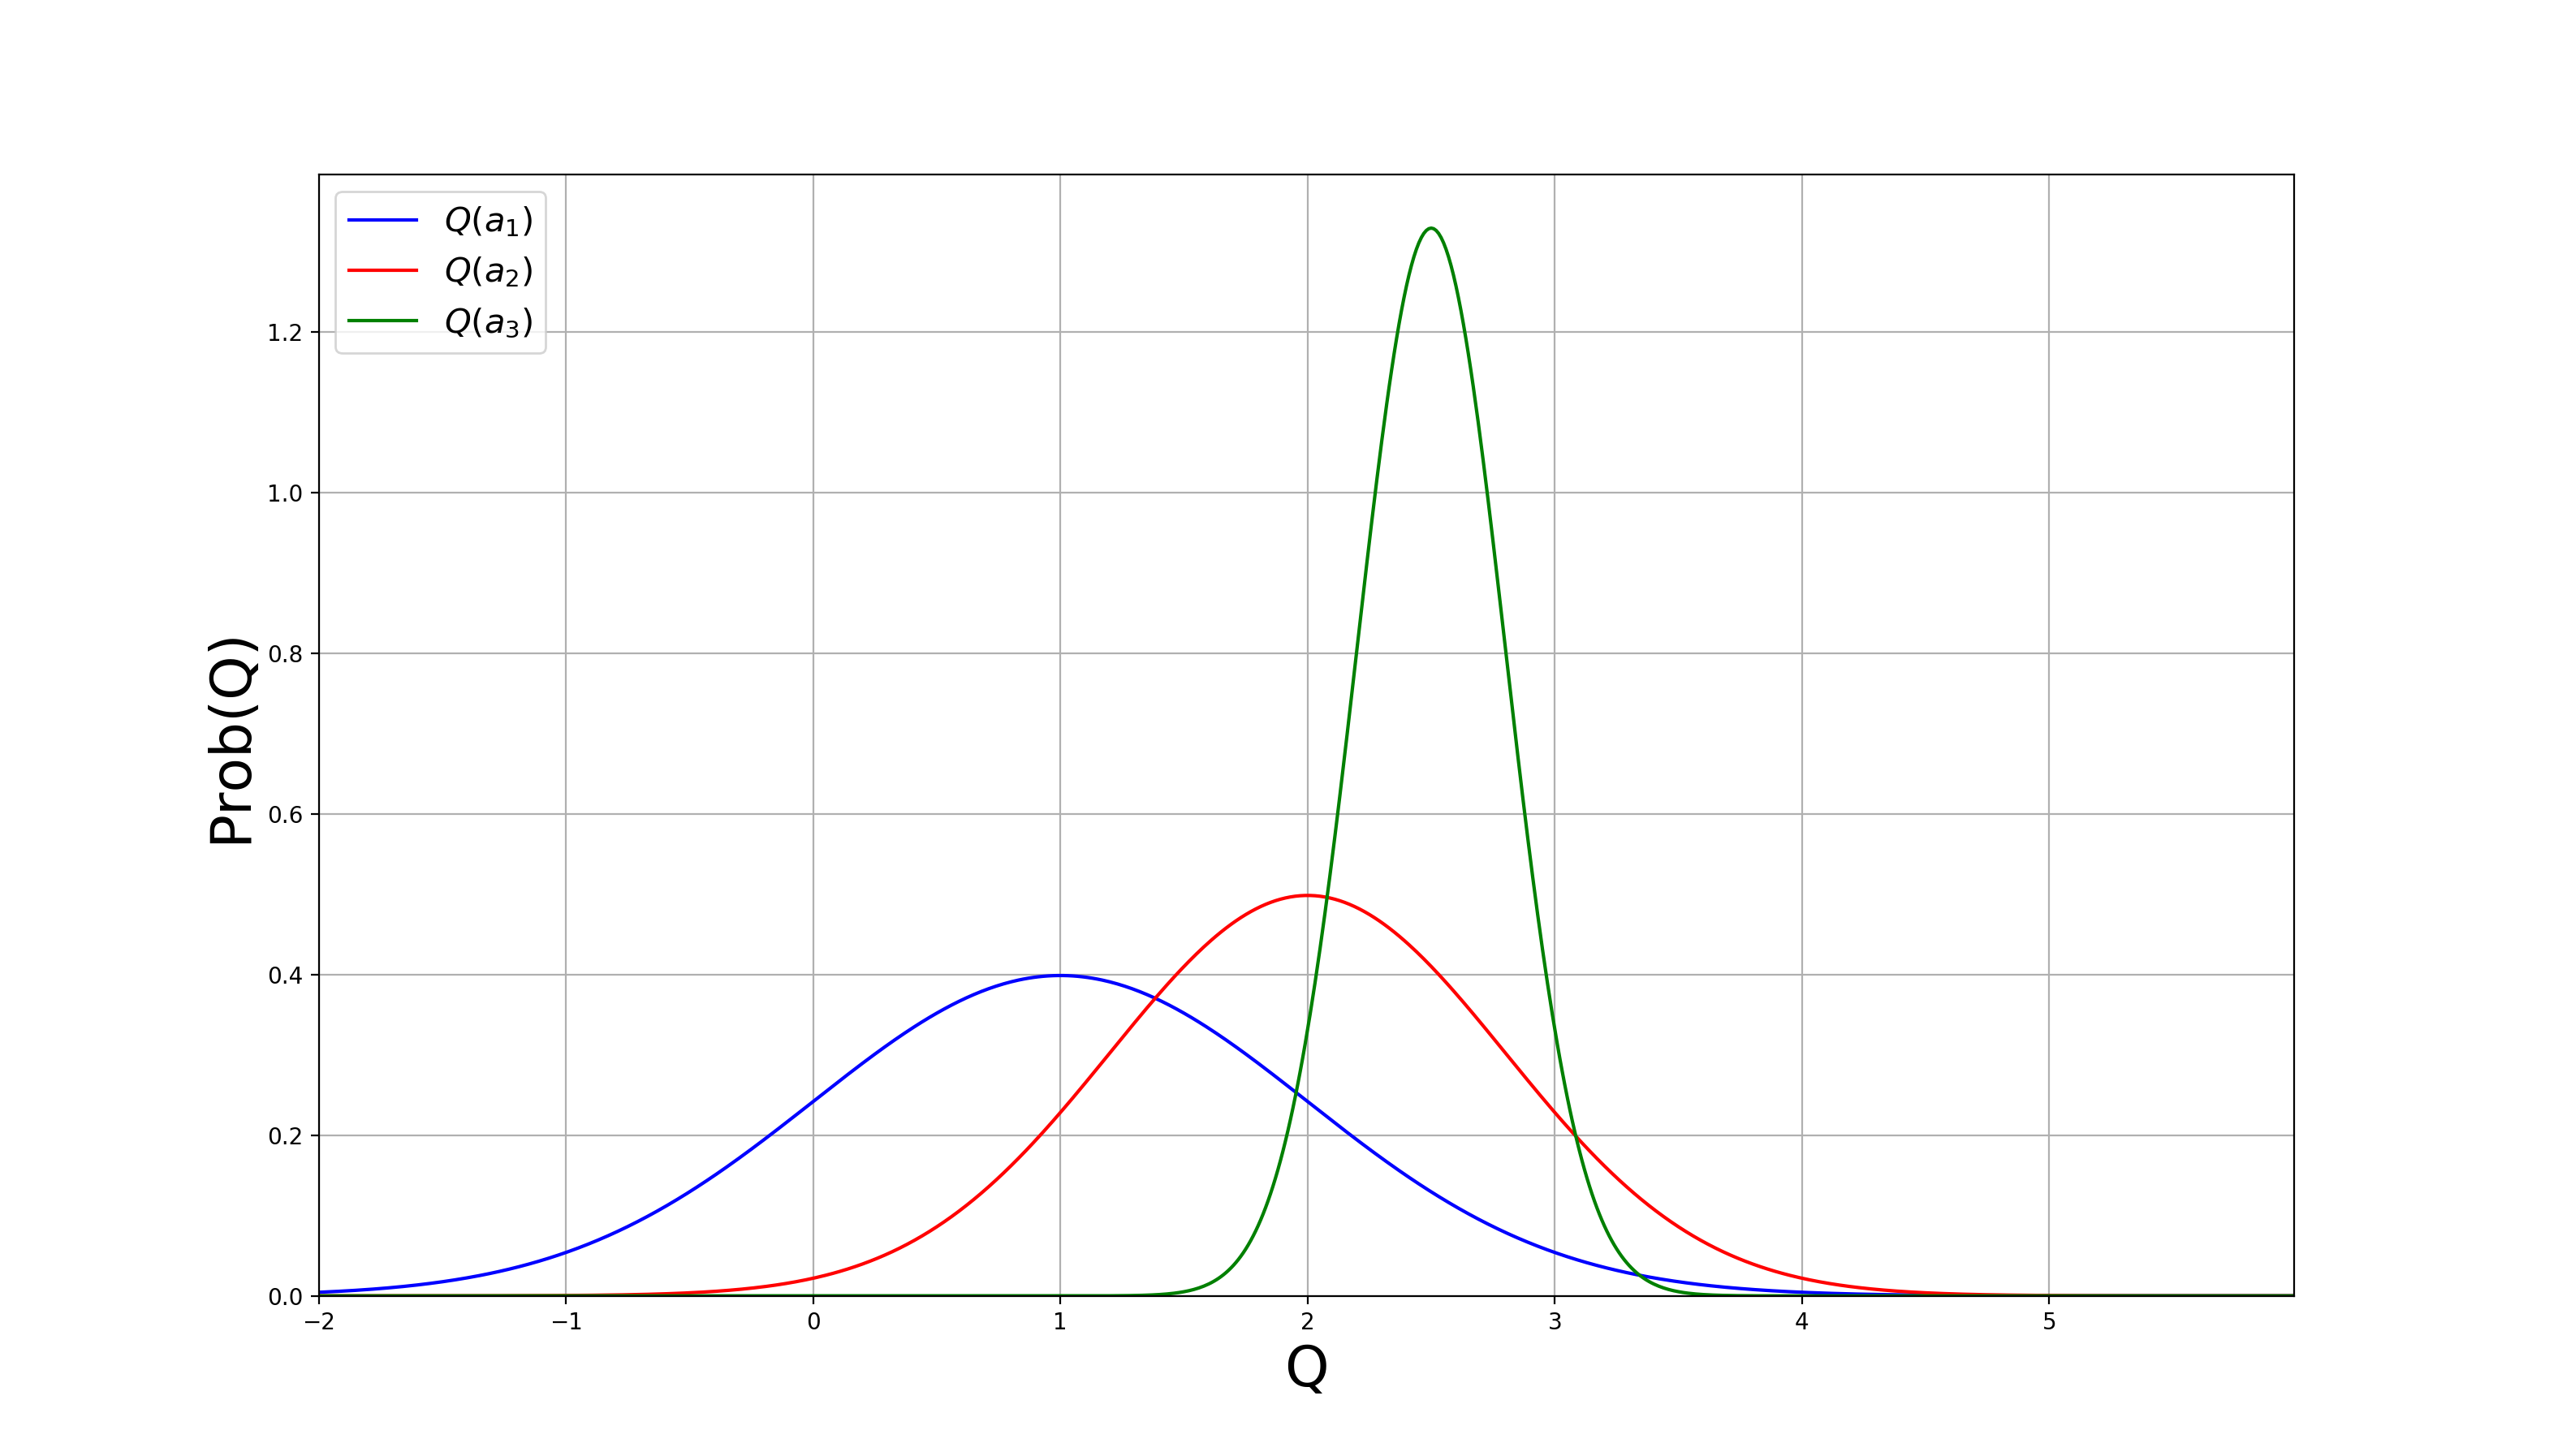
\includegraphics[width=0.62\textwidth,height=0.52\textheight,keepaspectratio]{images/bandits/figures/uncertainty-2.jpg}
\begin{itemize}
    \item After picking \emph{blue}, we are less uncertain about its value
    \item And more likely to pick another action --- until we home in on the best
\end{itemize}
\end{frame}

\begin{frame}{Upper Confidence Bounds (UCB)}
\begin{itemize}
    \setlength{\itemsep}{0.45em}
    \item Two things per arm: $Q(a)$, the \emph{true} mean we can never see, and $\hat{Q}_t(a)$, our \emph{sample-mean estimate} of it after $N_t(a)$ pulls
    \item Idea: be optimistic --- add a margin $\hat{U}_t(a)$ wide enough that the truth is very likely below it, then act on the sum:
    \[
        Q(a) \;\leq\; \underbrace{\hat{Q}_t(a)}_{\text{what we measured}} + \underbrace{\hat{U}_t(a)}_{\text{room for error}},
        \qquad a_{t+1} = \operatorname*{arg\,max}_{a} \big\{ \hat{Q}_t(a) + \hat{U}_t(a) \big\}
    \]
    \item $\hat{U}_t(a)$ is \emph{large} when $N_t(a)$ is small (we know little) and \emph{shrinks} as the arm is pulled more
    \item \textcolor{red}{So UCB never asks ``which arm \emph{is} best?'' --- it asks ``which arm \emph{could} be best?''} A barely-tried arm that currently looks bad still gets pulled, because its true value could plausibly still be high
\end{itemize}
\end{frame}

\begin{frame}{The UCB1 Algorithm}
\textbf{``UCB'' is the recipe; UCB1 fills it in} --- assume rewards bounded in $[0,1]$:
\[
    a_{t+1} = \operatorname*{arg\,max}_{a \in \mathcal{A}} \left\{ \hat{Q}_t(a) + \sqrt{\frac{\alpha \log t}{2 N_t(a)}} \right\}
\]
\begin{itemize}
    \setlength{\itemsep}{0.5em}
    \item \textcolor{gray}{The \emph{shape} is what matters: the bonus shrinks like $\mathbf{1/\sqrt{N_t(a)}}$ --- remember it, it reappears all afternoon}
    \item It grows slowly with the clock $t$, so an arm left alone long enough is revisited: exploration is \textbf{automatic}, no $\epsilon$ and no schedule
    \item \textbf{Unlike optimistic initialisation}, the bonus is recomputed \emph{every step} --- an arm unlucky early is never written off for good
    \item \textcolor{red}{Regret grows as $\mathcal{O}(\log T)$} (Auer et al., 2002) --- \textbf{sublinear at last}, provably the best possible rate. \href{https://github.com/TikhonJelvis/RL-book/tree/master/rl/chapter14/ucb1.py}{Educational Code}
\end{itemize}
\end{frame}

% --- Bayesian bandits: 2 slides merged into 1, Gaussian conjugacy dropped ---
\begin{frame}{Bayesian Bandits: Keep a Curve, Not a Number}
\vspace{-0.3em}
\begin{center}
\begin{tikzpicture}
\begin{axis}[
    width=0.80\textwidth, height=0.38\textheight,
    xlabel={\small this arm's true click rate}, ylabel={\small belief},
    xmin=0, xmax=1, ymin=0, ymax=9.6,
    ytick=\empty, xtick={0,0.3,0.5,1},
    axis lines=left, samples=200, domain=0:1,
    legend style={at={(0.99,0.99)},anchor=north east,draw=none,fill=none,font=\scriptsize},
    every axis plot/.append style={very thick},
]
\addplot[gray,dashed] {1};                        \addlegendentry{before any data}
\addplot[blue]  {1320*x^3*(1-x)^7};               \addlegendentry{10 shows, 3 clicks}
\addplot[red]   {1.617e14*x^15*(1-x)^35};         \addlegendentry{50 shows, 15 clicks}
\end{axis}
\end{tikzpicture}
\end{center}
\vspace{-0.3em}
\begin{itemize}
    \setlength{\itemsep}{0.3em}
    \item The curve is our \textbf{belief} about that one arm. Flat means ``could be anything'' --- that is the \textbf{prior}, and it is a complete answer to ``I know nothing''
    \item Each reward reshapes it into the \textbf{posterior}: the peak moves to what we have seen, and the curve \emph{narrows} as evidence piles up
    \item \textcolor{red}{The width \emph{is} the uncertainty} --- measured, not bounded from above like UCB's $\hat{U}$ --- and unlike a single number, a curve can be \emph{sampled} from
\end{itemize}
\end{frame}

% --- Thompson: 2 slides merged into 1, idea before the jargon ---
\begin{frame}{Thompson Sampling}
\textbf{One line:} draw a \emph{plausible} value for each arm from its curve; pull whichever wins the draw.
\vspace{-0.2em}
\begin{block}{The whole algorithm, for click / no-click rewards}
\vspace{-0.2em}
Per arm, \emph{two counters}: $s_a$ (clicks), $f_a$ (misses). Repeat:
\begin{enumerate}
    \item Draw $\theta_a \sim \mathrm{Beta}(1+s_a,\; 1+f_a)$ for every arm \hfill \textcolor{gray}{$\leftarrow$ that Beta \emph{is} the curve}
    \item Pull $a_t = \operatorname*{arg\,max}_a \theta_a$, and increment $s_{a_t}$ or $f_{a_t}$ by the outcome
\end{enumerate}
\vspace{-0.1em}
{\footnotesize\textcolor{gray}{No integrals anywhere --- the posterior \emph{is} those two integers.}}
\end{block}
\begin{itemize}
    \setlength{\itemsep}{0.3em}
    \item \textbf{Why this explores:} a barely-tried arm has a wide curve, so its draw is sometimes high --- and it gets pulled. A well-measured mediocre arm has a narrow curve and almost never wins
    \item \textcolor{red}{Same $\mathcal{O}(\log T)$ regret as UCB1}, usually better in practice; the standard bandit algorithm in production personalisation (Netflix, Lyft)
\end{itemize}
\centering\small\textcolor{gray}{Formally \emph{probability matching}. \href{https://github.com/TikhonJelvis/RL-book/tree/master/rl/chapter14/ts_bernoulli.py}{Bernoulli} / \href{https://github.com/TikhonJelvis/RL-book/tree/master/rl/chapter14/ts_gaussian.py}{Gaussian} code.}
\end{frame}
